%%%%%%%%%%Third Chapter%%%%%%%%%%
\chapter{Simulation Setup and Design}

\section{Overview}
This chapter describes the simulation setup and design procedure used in this thesis. The workflow starts from the definition of the design requirements, followed by the metasurface unit cell design, transmitarray lens configuration, antenna simulation setup, and communication channel evaluation. The simulation is intended to evaluate both the electromagnetic performance of the antenna and its influence on the communication channel.

\begin{figure}[h!]
	\centerline{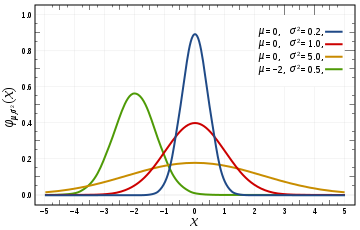
\includegraphics[width=0.65\textwidth]{Images/gambar.png}}
	\caption{Example simulation-related figure for Chapter 3}
	\label{fig:chapter3_simulation_example}
\end{figure}

\section{Design Requirements}
The design requirements define the target performance and simulation scope. The main parameters include operating frequency, aperture size, feed position, focal distance, polarization, desired beam direction, gain target, and channel evaluation scenario. These requirements are used as the basis for the transmitarray lens design and the communication link evaluation.

\section{Metasurface Unit Cell Design}
The metasurface unit cell is designed to provide the required transmission phase response while maintaining acceptable transmission magnitude. Each unit cell geometry is simulated to obtain its transmission coefficient, phase response, and operating bandwidth. The unit cell response is then used to determine the phase compensation required across the transmitarray aperture.

\subsection{Unit Cell Boundary Condition}
Periodic boundary conditions are used to represent an infinite metasurface array during unit cell simulation. The incident wave is applied to the unit cell, and the transmitted response is observed at the output port. This setup allows the phase and magnitude response of one unit cell to be evaluated efficiently.

\subsection{Transmission Phase Response}
The transmission phase response is the main design parameter for the transmitarray lens. A suitable unit cell should provide a wide phase tuning range with low transmission loss. The selected unit cell dimensions are mapped to the required phase distribution of the aperture.

\section{Transmitarray Lens Design}
The transmitarray lens is formed by arranging unit cells over a planar aperture. Each unit cell is assigned a phase shift based on its position relative to the feed antenna. The purpose of the lens is to compensate for the feed path difference and produce a desired transmitted wavefront.

\subsection{Feed Antenna Configuration}
The feed antenna is placed at a selected focal distance from the transmitarray aperture. The feed position determines the incident phase distribution on the lens surface. Proper feed placement is important to achieve efficient aperture illumination and reduce spillover loss.

\subsection{Phase Compensation Distribution}
The phase compensation distribution is calculated from the path length between the feed antenna and each unit cell position. The required phase is then converted into a corresponding unit cell geometry. This process determines the final layout of the metasurface transmitarray lens.

\section{ANSYS HFSS Simulation Setup}
ANSYS HFSS is used to evaluate the electromagnetic performance of the antenna design. The simulation setup includes material definition, geometry construction, excitation, boundary conditions, radiation region, meshing configuration, and frequency sweep. The antenna performance is evaluated using parameters such as S-parameters, gain, directivity, radiation pattern, and aperture behavior.

\subsection{Material and Geometry Definition}
The substrate, conductor, and surrounding air region are defined based on the selected antenna structure. The unit cell and transmitarray aperture geometry are constructed according to the final design dimensions.

\subsection{Excitation and Boundary Condition}
The excitation is assigned according to the antenna feeding structure. Radiation or open boundary conditions are applied around the simulation domain to represent free-space propagation. For unit cell simulation, periodic boundaries are used, while for full antenna simulation, an open radiation region is applied.

\subsection{Frequency Sweep and Mesh Setup}
The frequency sweep is configured around the operating frequency to observe antenna performance across the target bandwidth. Mesh refinement is applied to ensure that the electromagnetic field distribution and radiation characteristics are accurately captured.

\section{Communication Channel Evaluation Setup}
The communication channel evaluation is used to observe how the antenna performance affects the communication link. The antenna radiation pattern, gain, and beam direction are used as input parameters for channel evaluation. The channel is assessed using link-related quantities such as received power, path loss, coverage, and signal-to-noise ratio.

\subsection{Evaluation Scenario}
The evaluation scenario defines the transmitter position, receiver position, propagation distance, antenna orientation, and surrounding environment. This scenario is used to compare the channel behavior under different antenna or propagation conditions.

\subsection{Ray Tracing or Hybrid Evaluation}
Ray tracing or a hybrid HFSS-based evaluation can be used to estimate the communication channel. In the hybrid approach, HFSS provides accurate antenna characteristics, while the propagation evaluation estimates how the radiated wave reaches the receiver. This allows antenna-level results to be connected with communication channel performance.

\subsection{Channel Performance Metrics}
The main channel performance metrics include path loss, received power, signal-to-noise ratio, delay spread, angular spread, and coverage area. These metrics are used to evaluate whether the designed antenna improves the communication link in the selected scenario.

\section{Simulation Workflow}
The complete simulation workflow is summarized as follows. First, the design requirements are defined. Second, the unit cell is simulated and optimized. Third, the transmitarray lens phase distribution is calculated and implemented. Fourth, the full antenna is simulated in HFSS. Finally, the antenna results are used to evaluate the communication channel performance.
